% Preamble
\documentclass[a4paper, 12pt]{article}
\usepackage[margin=1in]{geometry} % Set margin
\usepackage{pdfpages} % Insert pdf pages
\usepackage{amssymb,amsmath,amsthm, amsfonts} % Math libraries

% Line spacing
\usepackage{setspace}
\setstretch{1.4}

% Custom commands
\newcommand{\sub}[1]{\subsection{\underline{#1}}}
\renewcommand{\qed}{\ensuremath{\blacksquare\pagebreak}}
\renewcommand{\b}[1]{\textbf{#1}}
\renewcommand{\because}[1]{~\b{(#1)}\\}
\renewcommand{\d}{\ensuremath{\Downarrow\\~}}

% Set section point after number
\usepackage{titlesec}
\titlelabel{\thetitle.\quad}

% Begin Document %
\begin{document}


% Title Page
\begin{titlepage}
    %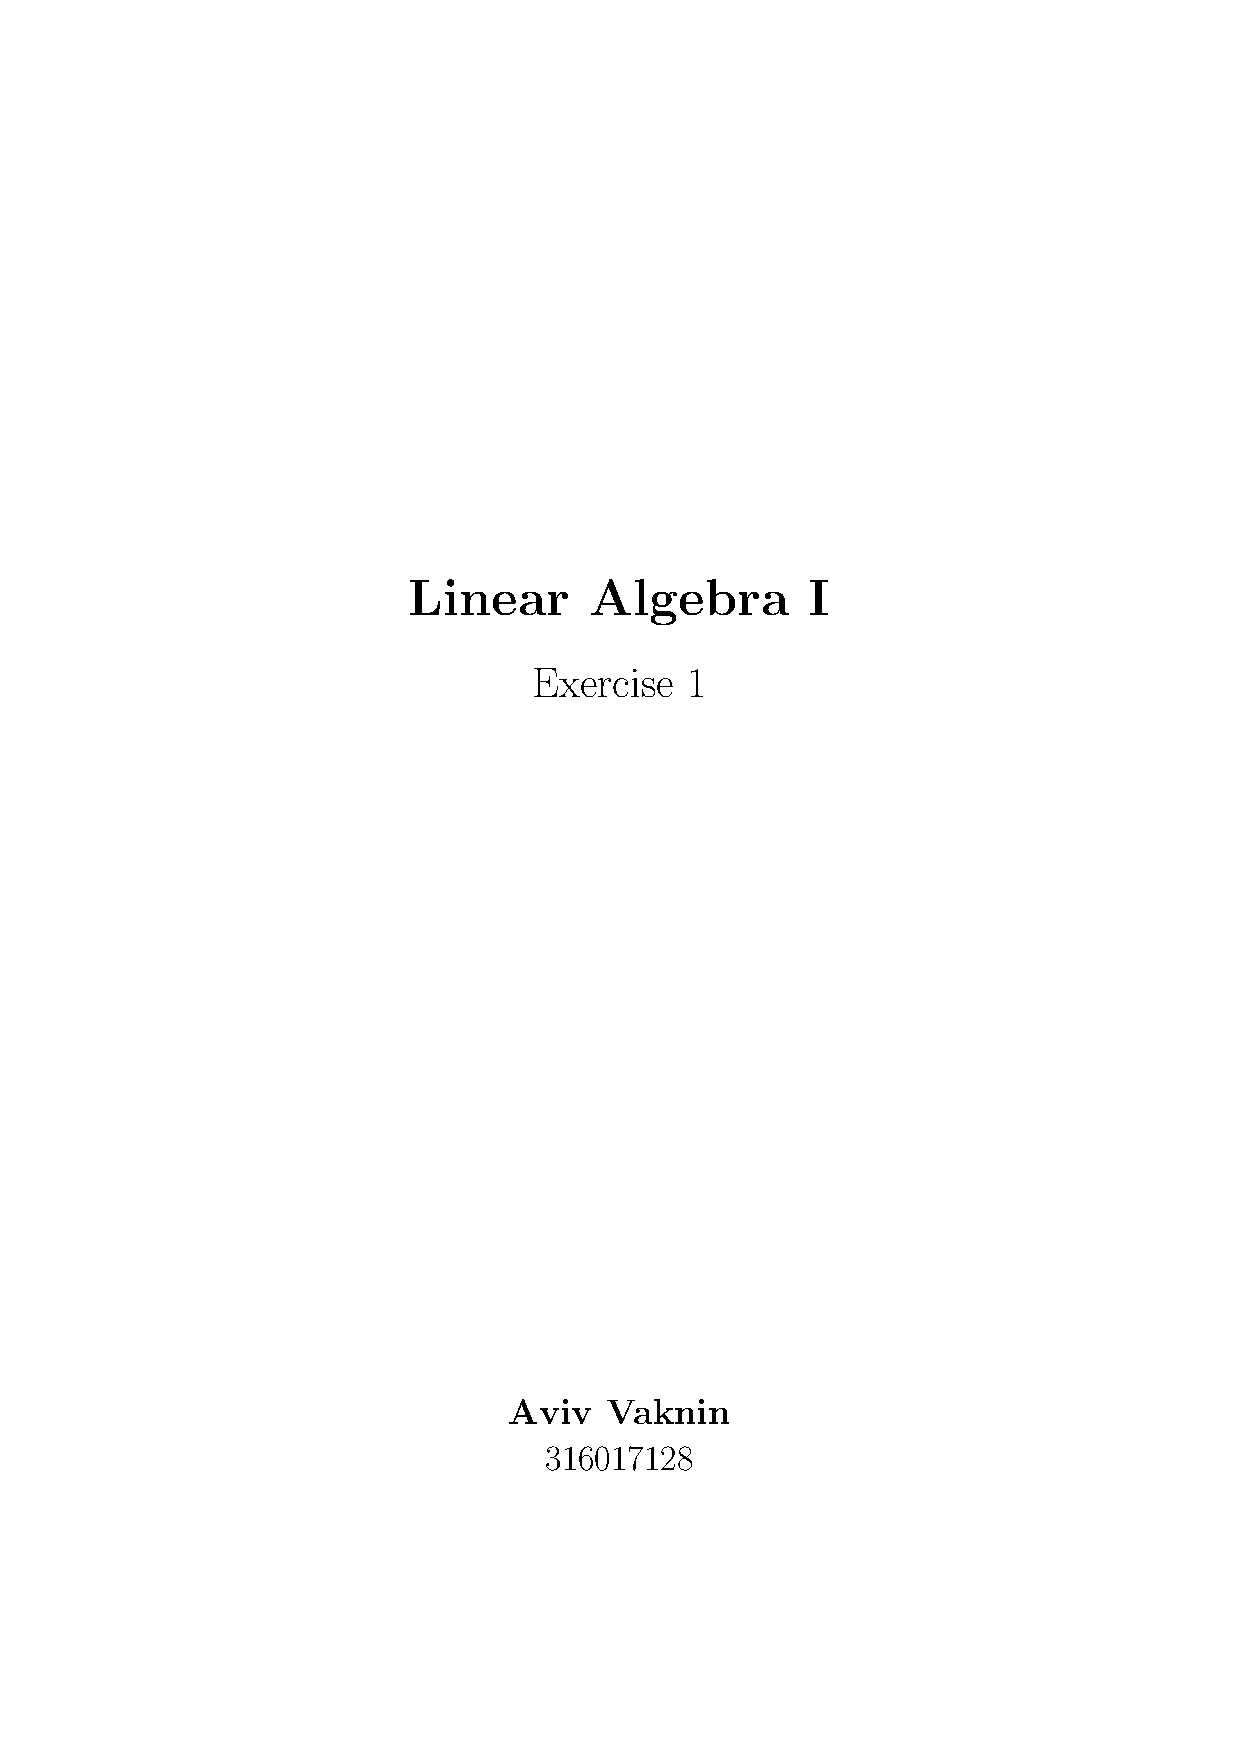
\includepdf{title.pdf}
\end{titlepage}

% 1
\section{What requirements S must fullfil in order to become a field?}
\begin{onehalfspace}
    In order to show that $S$ is a field, we'll need to prove the following \textit{\textbf{binary operator}} properties:
    \begin{enumerate}
        \item In $S$, there are two members, zero - $0_S$ and one - $1_S$
        \item $S$ supports the addition and multiplication binary operators
        \item Every member in $S$ can be negated, i.e. for every $x$ there is $-x$
        \item For every member in $S$ that is not $0_S$, $\exists{x^{-1}}\in{S}$, it is called the multiplicative inverse of $x$
    \end{enumerate}
    In addition, the mentioned binary operators should satisfy the following properties, referred to as \textit{\textbf{field axioms}}:
    \begin{enumerate}
        \item Associativity of addition(A1) and multiplication(M1):
            $$ a+(b+c)=(a+b)+c $$
            $$ a\cdot(b\cdot{c})=(a\cdot{b})\cdot{c} $$
        \item Commutativity of addition(A2) and multiplication(M2):
            $$ a+b = b+a $$
            $$ a\cdot{b} = b\cdot{a} $$
        \item Additive identity(A3) and multiplicative identity(M3)
            $$ a+0=a $$
            $$ a\cdot{1}=a $$
        \item Additive inverse(A4) and multiplicative inverse(M4)
            $$ a + (-a) = 0 $$
            $$ a \cdot a^-1 = 1 $$
        \item Distributivity(D)
            $$ a(b + c) = (a \cdot{b})+(a \cdot{c}) $$
    \end{enumerate}
\end{onehalfspace}
\pagebreak

% 2
\section{Prove: $ ((a + b) + c) + d = (a + b) + (c + d) = a + (b + (c + d)) $}
\subsection{$ \underline{((a+b)+c)+d=(a+b)+(c+d)}: $}
let $h=(a+b)$\\
$(h+c)+d=((a+b)+c)+d$\\
$(h+c)+d = h+(c+d)$\because{A1}
$ h+(c+d) = (a+b)+(c+d) $ \\
\d
$((a+b)+c)+d=(a+b)+(c+d)$
\subsection{$ \underline{ a+(b+(c+d))=(a+b)+(c+d) }: $}
let $h=(c+d)$\\
$ a+(b+h) = a+(b+(c+d)) $\\
$ a+(b+h) = (a+b)+h $\because{A1}
$ (a+b)+h = (a+b)+(c+d) $ \\
\d
$ a+(b+(c+d)) = (a+b)+(c+d) $\\
\qed

% 3
\section{Prove: $ \forall{x,y}\in{F},~x(y-z) = xy-xz $}
$ x(y-z) = x(y+(-z)) $\because{A1}
$ x(y+(-z)) = (x\cdot{y})+(x\cdot(-z))$\because{D}
$ (x\cdot{y})+(x\cdot(-z)) = (x\cdot{y})+(-x\cdot{z})) = (x\cdot{y})-(x\cdot{z})) $\\
$ (x\cdot{y})-(x\cdot{z})) = xy - xz $\\
\qed

% 4
\section{Prove: $ \forall{x,y}\in{F},~ (x+y)(x+y) = xx + xy + yx + yy $}
let $ h=(x+y) $\\
$
    (x+y)(x+y) = h\cdot(x+y)\\
    h\cdot(x+y) = (x\cdot{h})+(y\cdot{h}) = x(x+y) + y(x+y) \because{D}
    x(x+y) + y(x+y) = xx + xy + yx + yy \because{D}
$
\qed

% 5
\section{Prove: $ \forall{x,y}\in{F},~ (x+y)(x-y) = xx - yy $}

$
    (x+y)(x-y) = xx - xy + yx - yy \because{ex. 4}
    xx - xy + yx - yy = xx + (-xy + yx) - yy \because{A1}
    (-xy + yx) = (-xy + xy) \because{A2}
    (-xy + xy) = 0 \because{A4}
    \d
    xx + (-xy + yx) - yy = xx + 0 - yy = xx - yy \because{A3}
$
\qed

% 6
\section{Prove: $ (a=b) \land (c=d) \Rightarrow (a+c=b+d) \land (ac=bd) $}

\sub{$ (a=b) \land (c=d) \Rightarrow a+c=b+d $:}
$
    c=d=x \\
    a=b \\
    a+x=b+x \because{Consistency with addition}
    a+x=a+c \because{x=c}
    b+x=b+d \because{x=d}
    \d
    a+c=b+d\\
$

\sub{$ (a=b) \land (c=d) \Rightarrow ac=bd $:}
$
    c=d=x \\
    a=b \\
    ax=bx \because{Consistency with multiplication}
    ax=ac \because{x=c}
    bx=bd \because{x=d}
    \d
    ac=bd\\
$
\qed

% 7
\section{$ A=\bigg{\{} \dbinom{1}{a} \bigg{|} a\in{\mathbb{R} }\bigg{\}} $}
\sub{Does A have a neutral additive member?}
$
    \dbinom{1}{a} \oplus \dbinom{1}{0} = \dbinom{1}{a+0} \\
    \dbinom{1}{a+0} = \dbinom{1}{a} \because{A3}
    \d
    0_{A} = \dbinom{1}{0}
$

\sub{Does A have a neutral multiplicative member?}
$
    \dbinom{1}{a} \odot \dbinom{1}{1} = \dbinom{1}{a \cdot{1}} \\
    \dbinom{1}{a \cdot{1}} = \dbinom{1}{a} \because{M3}
    \d
    1_{A} = \dbinom{1}{1}
$

\sub{Is A a field?}


% End Document %
\end{document}